
\documentclass[runningheads]{llncs}
\usepackage{graphicx}
\usepackage{apacite}
\usepackage{float}
\usepackage{listings}
\usepackage{float}
\usepackage[table]{xcolor}
\usepackage[toc,page]{appendix}
\usepackage{ucs}
\usepackage[utf8x]{inputenc}

\usepackage[slovene]{babel}
\selectlanguage{slovene}


\lstset{
    breaklines=true,
    breakatwhitespace=true,
    inputencoding=utf8,
    extendedchars=false,
}


\renewcommand{\baselinestretch}{1.2} % za boljšo berljivost večji razmak
\renewcommand{\appendixpagename}{\normalfont\Large\bfseries{Appendix}}




\begin{document}

\title{Programming Assignment 2}
\subtitle{Implementing structured data extraction}

\author{
  Jaka Kokošar
  \and
  Danijel Maraž
  \and
  Toni Kocjan
}


\institute{Fakulteta za Računalništvo in Informatiko UL
\email{dm9929@student.uni-lj.si, jk0902@student.uni-lj.si, tk3152@student.uni-lj.si}\\
}

\maketitle             

\begin{abstract}
The article covers the work done in the scope of the second programming assignment as part of the subject web information extraction and retrieval. 

\keywords{Data Extraction Retrieval XPath Regex Roadrunner }
\end{abstract}

\section{Introduction}
After having collected the raw data with a crawler the logical next step is to convert it into a more structured format. As web pages do not have a strict shape this poses quite a challenge as any attempt of data extraction must be robust and resistant to various deformities in the html code. The report covers our attempts in implementing processes of structured data extraction in 6 different pages using basic methods such as regular expressions and xpath expressions. Alongside this an attempt was made to implement the RoadRunner algorithm which greatly simplifies the unpredictability aspect of data extraction.
\section{Description of chosen web pages and data items}
In addition to the mandatory websites, we selected a PZS\footnote{\url{https://www.pzs.si/}} ({\em Planinska zveza Slovenije}) site, which is the central register of information about the operation of mountain huts in Slovenia. As shown in Figure \ref{fig:Slika1}, we wanted to extract information of accommodations, location and contact details of a given hut. Since there are no other resources or APIs through which we could access this information and use them for any other purpose, we are forced to obtain information directly from this site.

\begin{figure}[H]
\begin{center}
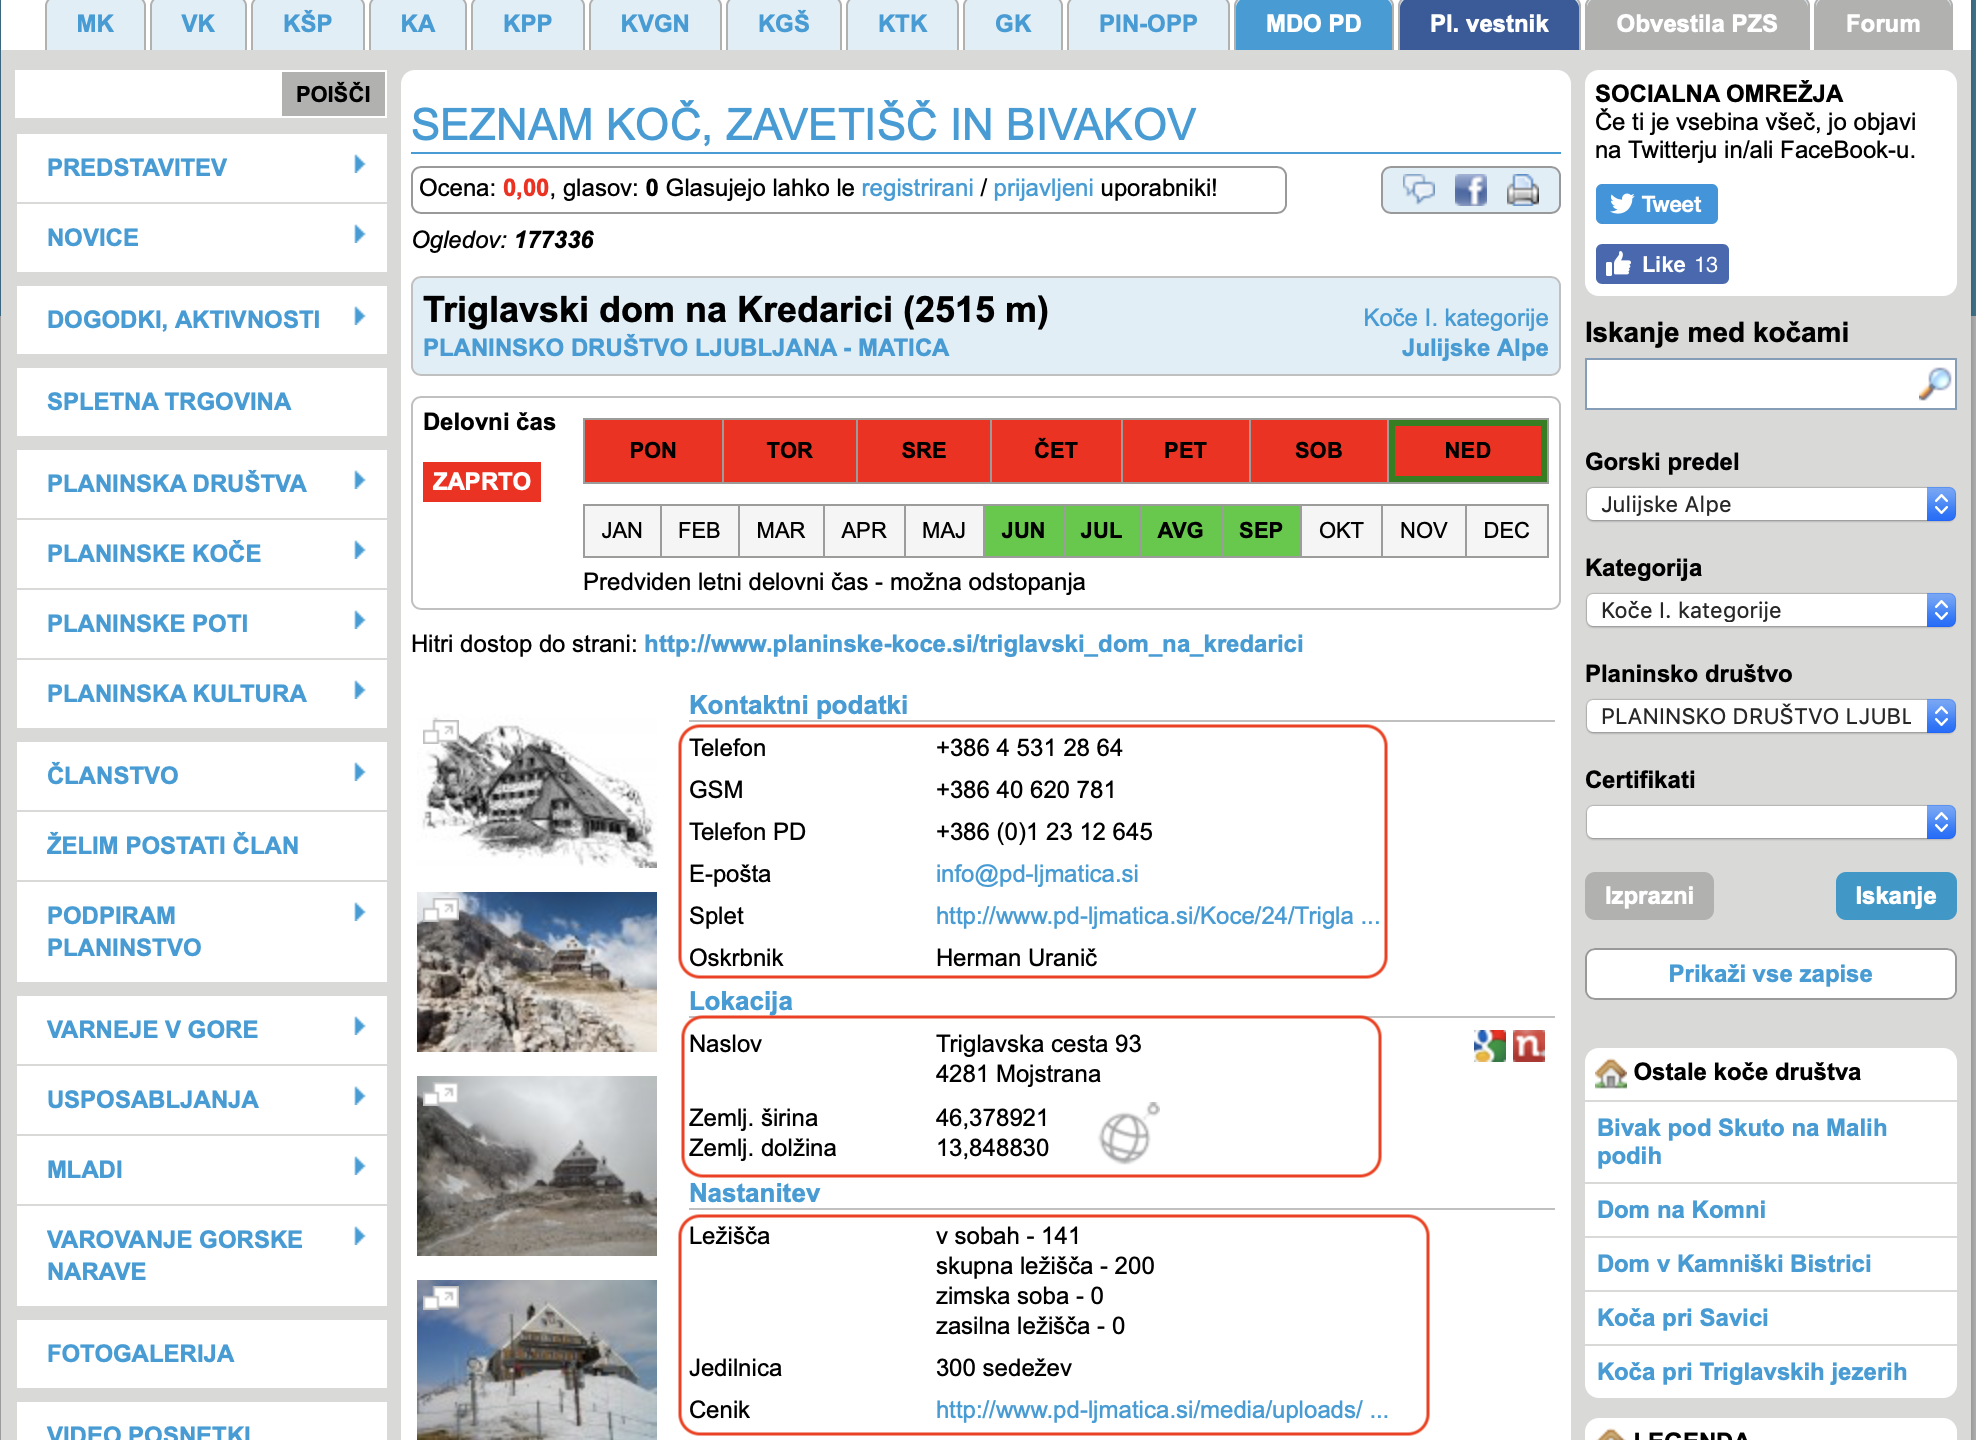
\includegraphics[scale=0.4]{pzs.png}
\caption{Data items we want to extract from pzs.si website}
\label{fig:Slika1}
\end{center}
\end{figure}

\section{Regular expressions implementation}
We defined three functions {\em parse\_rtv\_content},  {\em parse\_overstock\_content},  {\em parse\_pzs\_content}. Every function is responsible for a different page type but they are structured similarly. We extract data in three steps:
\begin{enumerate}
   \item read the input file
   \item pattern matching
   \item clean the results
\end{enumerate}
We only define one regular expression per page type. We extract all of the data items with a single expression in which we define all of the desired groups. After we obtain the results we clean the data of leftover html tags and strip newlines, whitespaces and tabulators. Results are available in the project repository\footnote{\url{https://github.com/LampDM/structured\_data\_extraction\_methods/tree/master/output/regex}}.

\section{XPath implementation}

\subsection{Jewelry}
An initial Xpath expression is called on the input html which selects a \textit{tbody} element. The children of this element represent our jewelry and other items on the page. We count the number of children and with a for loop and extra Xpath expression access each data item that interests us for each child. Any children that are malformed or do not contain the items we're interested in (such as price etc.) encounter an exception as the Xpath expression throws an error and is automatically not processed. Afterwards some minor post-processing of the acquired strings is done and the json is created.

\subsection{Cars}
The items Title, SubTitle, Author, PublishedTime and Lead are all collected via seperate XPath expressions on the input html as both pages have the same structure when it comes to them. The main difference between the two pages is the structure of the article body from which we've derived our Content item. We handle this by first extracting an article body tag which contains all the contents we need. Afterwards we give the extracted element as an argument to our function \textit{intr} which recursively iterates through the tag structure and appends all encountered text into a \textit{nonlocal} string. The string is then briefly processed and added to our json output.

\subsection{Koce}
The two chosen pages are quite similar with the subtle difference of TODO

\section{RoadRunner like implementation}
\begin{lstlisting}
import numpy as np
 
def incmatrix(genl1,genl2):
    m = len(genl1)
    n = len(genl2)
    M = None #to become the incidence matrix
    VT = np.zeros((n*m,1), int)  #dummy variable
 
    #compute the bitwise xor matrix
    M1 = bitxormatrix(genl1)
    M2 = np.triu(bitxormatrix(genl2),1) 
 
    for i in range(m-1):
        for j in range(i+1, m):
            [r,c] = np.where(M2 == M1[i,j])
            for k in range(len(r)):
                VT[(i)*n + r[k]] = 1;
                VT[(i)*n + c[k]] = 1;
                VT[(j)*n + r[k]] = 1;
                VT[(j)*n + c[k]] = 1;
 
                if M is None:
                    M = np.copy(VT)
                else:
                    M = np.concatenate((M, VT), 1)
 
                VT = np.zeros((n*m,1), int)
 
    return M
\end{lstlisting}



\end{document}
